%%%%% Document Setup %%%%%%%%

\documentclass[12pt, twocolumn]{report}%{revtex4}    % Font size (12pt) and column number (one or two).

\usepackage{times}  % Times New Roman font type

\usepackage{natbib}

\usepackage{authblk}

\usepackage[a4paper, left=2.5cm, right=2.5cm,
 top=2.5cm, bottom=2.5cm]{geometry}       % Defines paper size and margin length

\renewcommand{\baselinestretch}{1.15}     % Defines the line spacing

\usepackage[font=small,
labelfont=bf]{caption}                      % Defines caption font size and caption title bolded

\usepackage{graphics,graphicx,epsfig,ulem}	% Makes sure all graphics works
\usepackage{amsmath}                        % Adds mathematical features for equations
\usepackage{float}
\usepackage{amssymb}

\usepackage{ltxgrid}

\usepackage{etoolbox}                       % Customise date to preferred format
\makeatletter
\patchcmd{\frontmatter@RRAP@format}{(}{}{}{}
\patchcmd{\frontmatter@RRAP@format}{)}{}{}{}
%\renewcommand\Dated@name{}
\makeatother

\def\thesection{\arabic{section}}

\def\bibsection{\section*{References}}        % Position reference section correctly

%%%%% Document %%%%%
\begin{document}                     

\title{A Model for the Evolution of Quasars} 
\date{Submitted: \today{}}
\author{Joseph Carter}
\affil{\normalfont Level 4 Project, MPhys Physics with Astronomy\\ Supervisor: Professor T. Theuns\\ Department of Physics, Durham University}

%\begin{abstract}
 
%Abstract abstract abstract abstract abstract abstract abstract abstract abstract abstract abstract abstract abstract abstract %abstract abstract abstract abstract abstract abstract abstract abstract abstract abstract abstract abstract abstract abstract %abstract abstract abstract abstract abstract abstract abstract abstract abstract abstract abstract abstract abstract abstract %abstract abstract abstract abstract abstract abstract abstract abstract abstract abstract abstract abstract 

%\end{abstract}


\maketitle
%\thispagestyle{plain} % produces page number for front page
\onecolumngrid


\tableofcontents
\newpage
\twocolumngrid
%\let\toc@pre\relax
%\let\toc@post\relax


\section{Introduction}

Almost all central galaxies (galaxies that are not satellites) are believed to contain a supermassive black hole (SMBH) at their centre. When a SMBH begins to rapidly increase in mass from accretion, the energy released from matter falling onto the black hole (BH) can exceed the luminosity of its host galaxy. These types of SMBH are known as active galactic nuclei (AGN). The most luminous AGN, with luminosities ranging between $~10^{11} - 10^{15}L_\odot$, are called quasars. The evolution of the host galaxies' dark matter halos is well understood, but how this relates to the formation and evolution of quasars is not as well understood.\par

The aim of this project is to develop a model for the formation and evolution of quasars using a model for galaxy formation which includes feedback from stars and accreting black holes. This paper describes how the relation between the growth of SMBHs and the growth of their host galaxies can be used to determine the rate at which quasars are formed in the universe.

\subsection{Overview}

The remainder of this section contains descriptions of the EAGLE simulations, which were used to produce most of the data used in this project, the COLOSSUS python package for cosmology-related calculations, and it is shown that COLOSSUS can be used to produce halo mass functions which are a good fit for EAGLE data, as these are used in section 3 to estimate the formation rate of quasars.\par

Section 2 discusses the motivation for this model. It is shown that many high mass galaxies have their star formation inhibited by AGN feedback, implying that there is a relationship between the mass of the galaxy and the presence or absence of an AGN. This relationship is discussed in further detail in section 3, and it is shown that the evolution of halo mass in EAGLE can be used to estimate the formation rate of quasars.

\subsection{The EAGLE Simulations}

Unless stated otherwise, all of the plots in this paper were produced using data from the Virgo Consortium’s “Evolution and Assembly of GaLaxies and their Environments” simulation suite (EAGLE) (\cite{EAGLE}). This is a set of cosmological hydrodynamical simulations which use a modified version of the GADGET smoothed particle hydrodynamics code (\cite{GADGET}). All plots were produced using the Ref-L0100N1504 simulation. Full details of the parameters used in the simulations can be found in the EAGLE paper. In EAGLE, halos that exceed a certain mass are given a 'seed' SMBH with an initial mass of $10^5M_\odot$.

\subsection{COLOSSUS}

Some plots in this paper were also produced using COLOSSUS (\cite{COLOSSUS}). This is a Python package for calculations related to cosmology, the large-scale structure of matter in the universe, and the properties of dark matter halos. In particular, it is used in this project to produce halo mass functions, as well as calculating the values of cosmological parameters, and converting between redshift and cosmic time. It is shown in the next section that the mass functions produced by COLOSSUS are a good fit for mass functions produced using data from EAGLE.

\subsection{Comparing the Halo Mass Functions of EAGLE and COLOSSUS}

\begin{figure}[H]
\centering
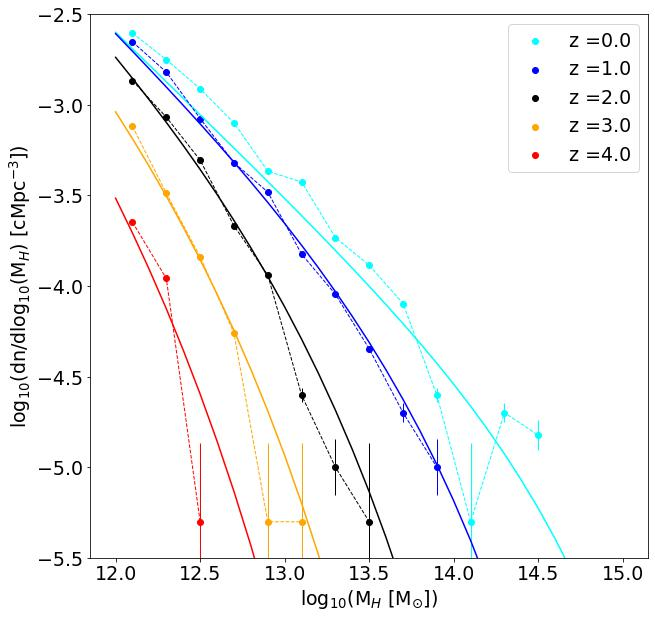
\includegraphics[width=\linewidth]{Mass_Function.jpeg}
\caption{Halo mass functions for galaxies of halo mass greater than $10^{12}M_\odot$ between z=0 and z=4. The dashed lines show mass functions from EAGLE, filled lines show mass functions from COLOSSUS, which have been converted to be in terms of $log_{10}(M_H)$ instead of their standard units of $ln(M_H)$ to match with units from EAGLE.}
\label{fig:1}
\end{figure}

Halo mass functions for EAGLE galaxies at various redshifts are plotted alongside halo mass functions from COLOSSUS in Fig.1 for comparison. The large uncertainties on the lower values of the EAGLE mass functions are due to the small number of high mass galaxies present in the simulation. It can be seen from Fig.1 that COLOSSUS produces mass functions that are a good fit for the measured mass functions from EAGLE. Additionally, the mass functions from COLOSSUS do not suffer from the same lack of measurable high mass galaxies as EAGLE, which is the cause for the large error in the EAGLE mass functions at higher masses, as seen in Fig.1.\par

As a result of these advantages, the comoving number density of halos of a given mass, plotted as a function of redshift, is used in section 3 to compute the rate at which galaxies transition from the blue cloud to the red sequence, and hence the rate at which quasars are formed as a function of redshift.

\section{The Effect of AGN Feedback on Star Formation}

The top plot of Fig.2 shows the relationship between u-r magnitude, which shows how blue (low magnitude) or red (high magnitude) an object is, and k-band magnitude, which is strongly correlated to stellar mass, for galaxies of mass greater than $10^9M_\odot$. It can be seen that the galaxy population in EAGLE is divided into a highly star forming "blue cloud" which contains the majority of galaxies with stellar mass below $10^{10}M_\odot$ and a "red sequence" with a significantly lower specific star formation rate (sSFR), which contains a significant amount of the high-mass galaxies (many of the galaxies in Fig.2 actually have an sSFR of 0, but have been equated to the lowest non-zero sSFR so that they can be shown on a log plot). The difference in star formation rate between the blue cloud and the red sequence is believed to depend on the type of feedback present in the galaxy. Star formation in blue cloud galaxies is regulated by  stellar feedback, in which the energy injected into the interstellar medium by supernovae balances the energy lost due to cosmological accretion (\cite{Ikea}).

\onecolumngrid


\begin{figure}[H]
\centering
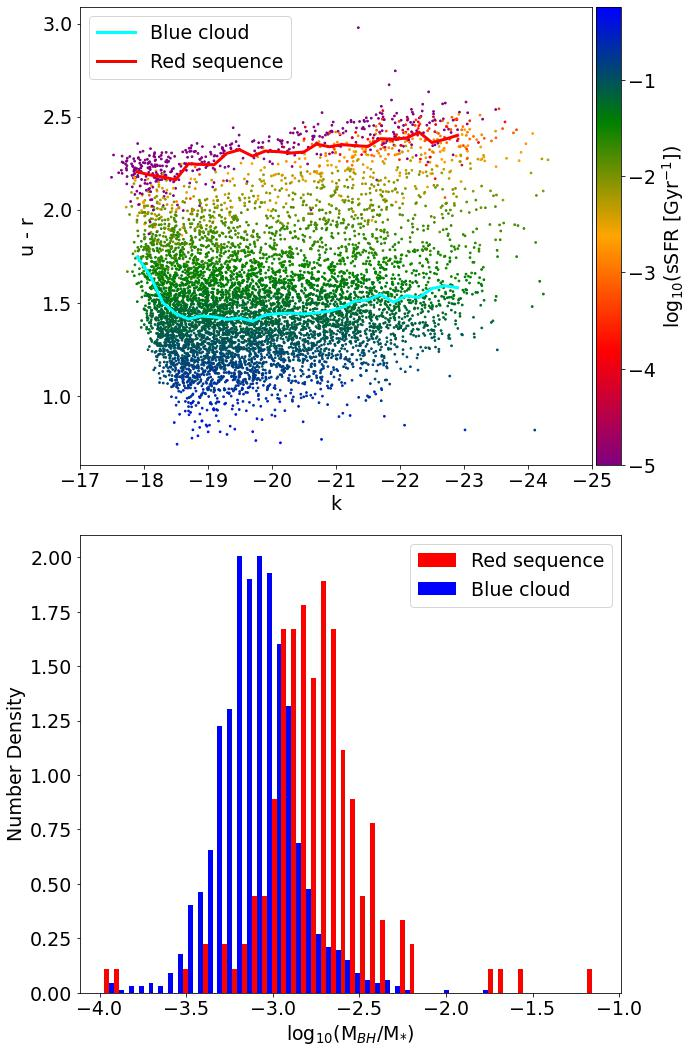
\includegraphics[width=15cm]{Plot_1.jpeg}
\caption{Top: u-r magnitude as a function of k-band magnitude for galaxies of stellar mass $\gtrsim10^9M_\odot$ at z=0. k-band magnitude is strongly correlated to stellar mass, so brighter galaxies can be taken to have higher stellar mass. Individual galaxies are plotted as points, coloured by sSFR, using the colourbar to the right. Bottom: Histogram of $M_{BH}/M_*$ for galaxies of stellar mass between $10^{10} - 10^{10.5}M_\odot$, separated into blue cloud galaxies and red sequence galaxies.}
\label{fig:2}
\end{figure}
\twocolumngrid

\noindent However, for galaxies with dark matter halos more massive than a critical mass of $M_{H,crit}\sim10^{12}M_\odot$ outflows driven by supernovae will no longer be buoyant, leading to a buildup of gas in the central regions of the galaxy. This allows the central black hole to grow rapidly, quickly reaching sufficient mass to begin AGN feedback, in which energy released by the black hole heats the gas corona surrounding the galaxy, disrupting the inflow of cold gas and suppressing star formation. More evidence of this can be seen from the colour of the points in Fig.3, as this shows a decrease in sSFR for galaxies with high BH mass and halo mass. The lower histogram of Fig.2 shows the difference in the ratio between BH mass and stellar mass for galaxies in the blue cloud and the red sequence. The histogram peaks at a higher value for the red sequence than for the blue cloud, implying that red sequence galaxies, on average, have a more massive BH compared to the mass of the host galaxy than for blue cloud galaxies. This provides further evidence that AGN feedback is responsible for the low star formation in the red sequence, as AGN are typically more massive than inactive SMBH's due to their high accretion rate.\par

\vspace*{1cm}

Since the presence of an AGN is believed to be the cause of galaxies making the transition from the blue cloud to the red sequence, measuring the number of galaxies which exceed $M_{crit}$ and therefore transition to the red sequence at a given redshift will also provide a measurement of the number of quasars formed at that redshift. This provides the motivation for our model, and is discussed further in the next section.

\vspace*{2cm}

\section{Relating Halo Mass to the Formation Rate of Quasars}
\subsection{The Black Hole Mass - Halo Mass Relation}

Fig.3 shows the black hole mass - halo mass relation for central galaxies of stellar mass $\gtrsim10^9M_\odot$. There appears to be little to no correlation at low halo masses, and the gaps with no points are due to black holes growing suddenly via mergers instead of continuously via accretion. For halo masses above $~10^{11.5}M_\odot$, black hole mass ad halo mass appear to be correlated. One problem when determining which black holes are accreting at close to the Eddington rate is that the instantaneous black hole accretion rates measured in EAGLE have a very large scatter, but it is known that halos increase in mass with cosmic time, so halos plotted on Fig.3 can be assumed to contain black holes that are growing according to the relation shown in Fig.3.\par

The right plot of Fig.3 shows that black hole mass follows an exponential fit for medium-mass halos, so halos that lie on the exponential curve (those between the vertical dotted lines) can be assumed to contain black holes that are growing exponentially, following the BH mass - halo mass relation, and halos that lie on the power law fit (those at higher masses than the exponential curve) can be assumed to contain black holes that are growing according to a power law. The exponential growth region seems promising for approximately Eddington limited black hole growth, but the black hole masses in this region are significantly lower than the measured masses of real quasars, which can have masses of $\sim10^9M_\odot$ (\cite{Marshall}). This could be a result of the approximation in EAGLE that all SMBHs start as seeds of a specific mass.

\onecolumngrid


\begin{figure}[H]
\centering
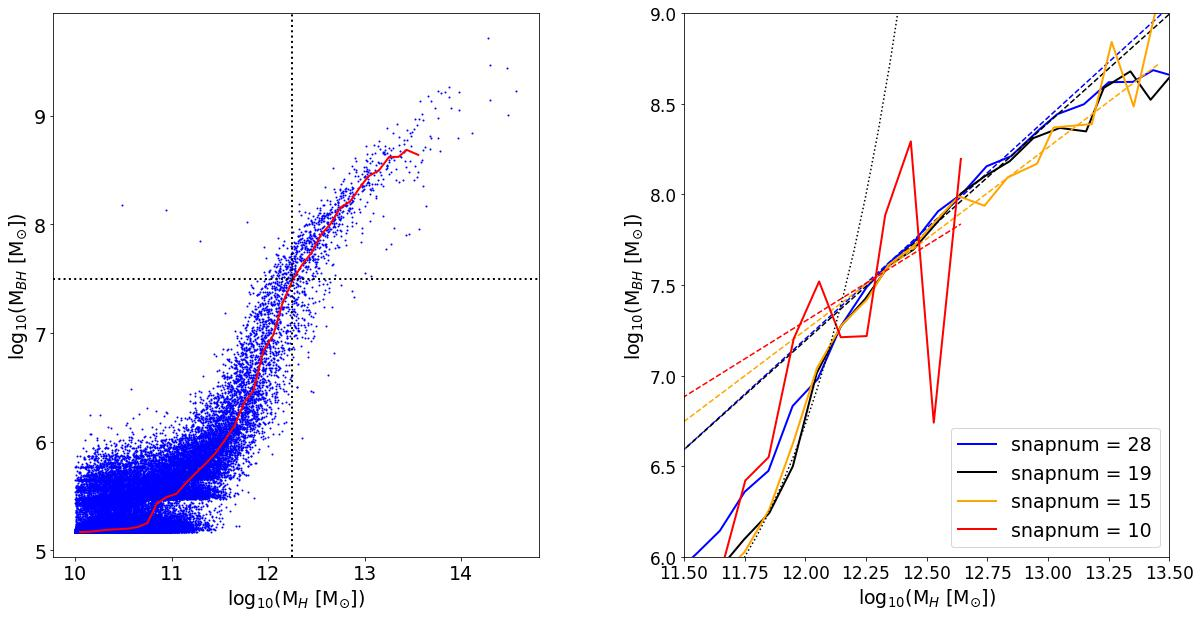
\includegraphics[width=17cm]{Plot_3.jpeg}
\caption{Left: Black hole mass - halo mass relation for central galaxies of stellar mass $\gtrsim10^9M_\odot$ at z=0, the blue line shows median black hole mass. Individual halos are plotted as points, coloured by sSFR, using the colourbar to the right. The dotted lines show BH mass (horizontal) and halo mass (vertical) at the beginning and end of the qso phase. Right: Median black hole mass as a function of halo mass for central galaxies at snapnums 28, 19, 15, and 10 (equivalent to z = 0, 1, 2, and 4 respectively). Dashed lines show power law fits, the dotted line shows an exponential fit.}
\label{fig:3}
\end{figure}
\twocolumngrid


 \noindent However, it is shown in \cite{Quasar} that the seed mass of the SMBHs has little effect on their final mass. Additionally, although the instantaneous BH accretion rates in EAGLE have a large scatter, it can be seen from Fig.4 that the Eddington ratios of the highest mass black holes do not appear to differ much from the Eddington ratios of $10^{6.5-7.5}M_\odot$ black holes. Therefore, the most luminous AGN should be the more massive black holes on the power law fit.\par

 \subsection{Calculating the Quasar Formation Rate}

The median black hole mass on the left plot of Fig.3 reaches a high enough BH mass for a luminous AGN at a halo mass of $\sim10^{12}M_\odot$. Our model assumes that the rate at which quasars are formed in EAGLE is equal to the rate at which galaxies cross the $10^{12}M_\odot$ halo 

\begin{figure}[H]
\centering
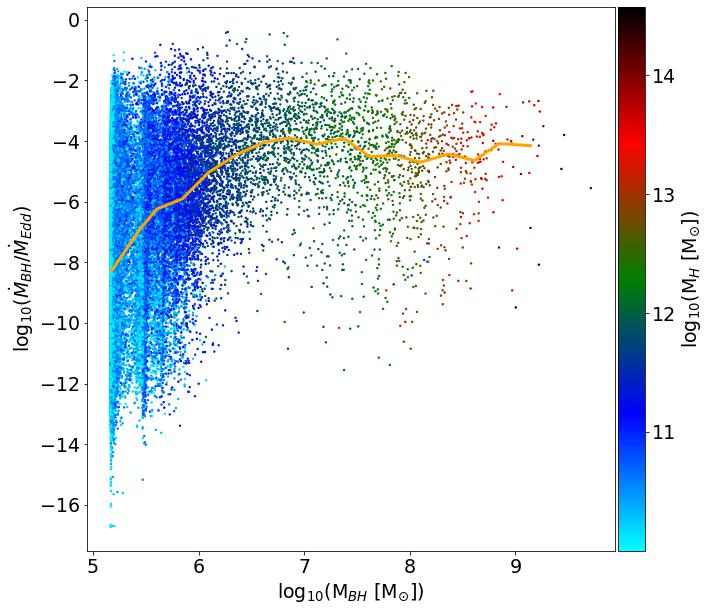
\includegraphics[width=\linewidth]{Plot_12.jpeg}
\caption{Instantaneous Eddington ratio - BH mass relation for halos more massive than $10^{10}M_\odot$. Individual halos are plotted as points, coloured by halo mass. The orange line shows median Eddington ratio, and appears to increase up to a BH mass of $\sim10^{6.5}M_\odot$, before its evolution stops.}
\label{fig:4}
\end{figure}

mass threshold: $dn/dz$, where n is the number of galaxies of halo mass greater than $10^{12}M_\odot$ per unit comoving volume. This can be calculated using (\cite{Correa})

\begin{equation}
    \frac{dn}{dz}=\frac{dn}{dln(M_H)}\frac{dln(M_H)}{dz}
\end{equation}

\noindent where $dn/dln(M_H)$ is the comoving number density of halos with mass $M_H=10^{12}M_\odot$ at a given redshift, which can be calculated from halo mass functions produced using COLOSSUS, and the logarithmic growth rate is given by

\begin{equation}
    \frac{dln(M_H)}{dz}=\frac{a}{(1+z)}-b
\end{equation}

\noindent This corresponds to the parametrisation described by \cite{Correa}, in which $M_H$ can be written as

\begin{align}
    \frac{M_H}{M_{H,0}}&=m_H(z) \nonumber \\
    m_H(z)&\approx(1+z)^ae^{-bz}
\end{align}

\noindent where a and b are fitting parameters, and $M_{H,0}$ is the value of $M_H$ at z=0. \cite{Correa}

\begin{figure}[H]
\centering
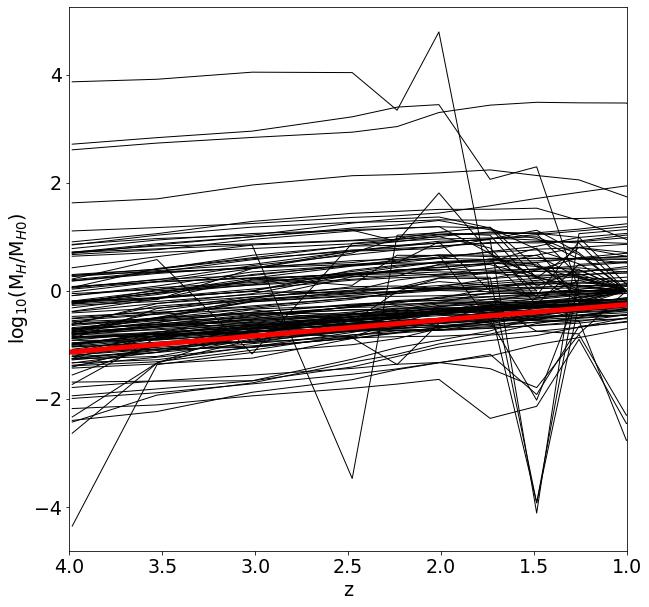
\includegraphics[width=\linewidth]{Plot_5.jpeg}
\caption{The black lines show $M_H/M_{H,0}$ as a function of redshift for central galaxies which cross the $10^{12}M_\odot$ halo mass threshold at z=2. The red line shows $M_H/M_{H,0}$ as described by Equation (3).}
\label{fig:5}
\end{figure}

\noindent gives values for a \& b, averaged over halo masses, as $\bar a \approx 0.24, \bar b \approx 0.75$, but to test their fit for the evolution of EAGLE galaxies crossing the $10^{12}M_\odot$ halo mass threshold, $M_H/M_{H,0}$ is plotted against z in Fig.5 for EAGLE galaxies and for $m_H(z)$. Fig.5 shows that Equation (3) fits the evolution of halo mass with redshift well for EAGLE galaxies crossing the $10^{12}M_\odot$ halo mass threshold (outliers in Fig.5 that are significantly more massive than they are at z=0 are believed to be caused by halos passing through one another and contributing to each others' measured masses, before moving away at $z\approx0$, leading to  sudden decreases in the measured value of $M_H$). This means that the constant values of $\bar a$ and $\bar b$ can be substituted into Equation (2)

\begin{equation}
    \frac{dln(M_H)}{dz}=\frac{\bar a}{(1+z)}-\bar b
\end{equation}

\noindent meaning that $dln(M_H)/dz$ and $dn/dln(M_H)$ are now functions of z only.\par

The top plot of Fig.6 shows the comoving number density of halos with mass $10^{12}M_\odot$, $dn/dln(M_H)$, for reference, and in the bottom plot, $dln(M_H)/dz$ and $dn/dln(M_H)$ are multiplied as in Equation (1) to produce a plot of the formation rate of halos with mass greater than $10^{12}M_\odot$, and hence the formation rate of quasars, $dn/dz$, as a function of redshift. The formation rate peaks at $z\approx1$ before decreasing for $1 \gtrsim z \geq 0$.

\onecolumngrid


\begin{figure}[H]
\centering
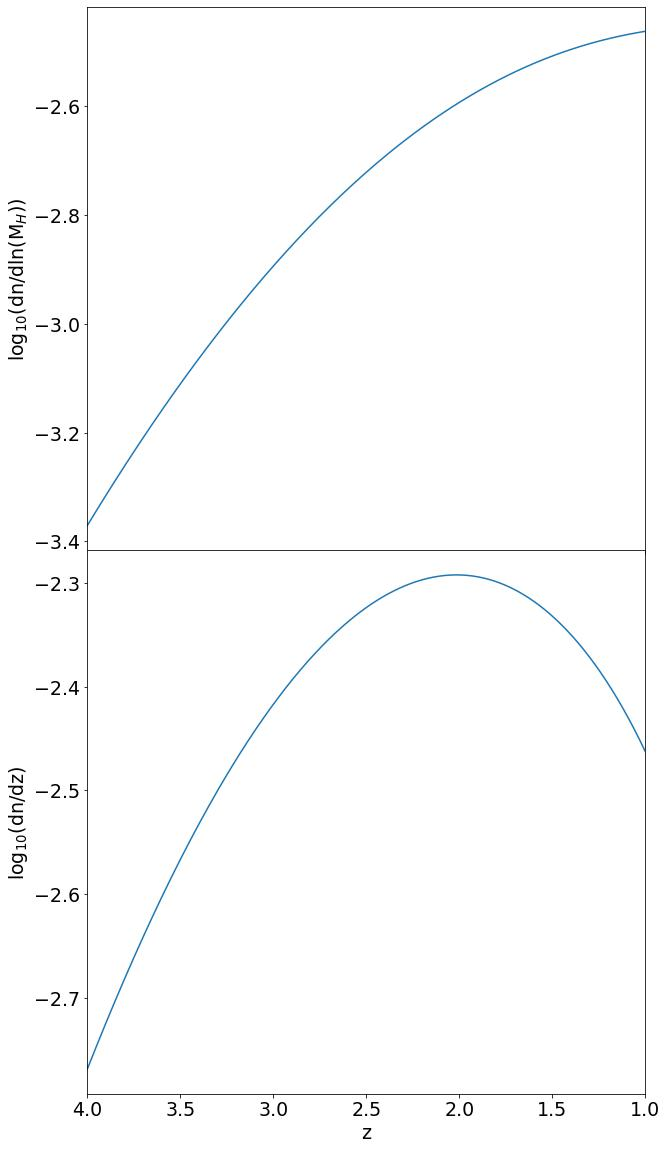
\includegraphics[width=12.5cm]{Plot_6.jpeg}
\caption{Top: Comoving number density of halos with mass $10^{12}M_\odot$ as a function of redshift, produced using COLOSSUS. Bottom: Formation rate of halos of mass greater than $10^{12}M_\odot$ as a function of redshift, calculated using Equation (2). This appears to peak at $z\approx1$.}
\label{fig:6}
\end{figure}
\newpage
\twocolumngrid


\section{Calculating Quasar Emissivity}

Our model now has a prediction for the formation rate of quasars, and the number density of quasars can be calculated from this, but these quantities are difficult to measure for the real universe. A measurable quantity which can also be calculated from this model is the quasar emissivity in a particular region of the EM spectrum, such as UV.\par

To obtain an estimate for quasar emissivity, the number density of quasars must first be calculated from the formation rate, and this in turn requires an estimate of the lifetime of each quasar. This section discusses how the quasar lifetime can be estimated, and then shows how the quasar emissivity can be calculated from this, and finally compares the results of these methods with quasar emissivity calculated by \cite{Haardt_Madau}.

\subsection{Calculating Quasar Emissivity in our Model}

The lifetimes of quasars are not very well understood. One possibility is that, since the black hole’s growth is driven by accreting material that falls into the centre of the halo, the quasar’s lifetime could be proportional to the dynamical timescale of the host halo.

\begin{equation}
    \tau\propto t_{dyn}=\frac{1}{\sqrt{G\rho}}
\end{equation}

\noindent This is the minimum time taken for a uniform gas cloud with density $\rho$ to collapse, and so would be approximately equal to the time taken for all the gas present in the halo at the start of the quasar phase to fall to the centre and drive the black hole’s accretion. By substituting $\Bar{\rho}_{halo}=200\Bar{\rho_{crit}}=200\frac{3H^2}{8\pi G}$ and rearranging, obtain

\begin{equation}
    t_{dyn}=\left(\frac{300}{4\pi}\right)^{-\frac{1}{2}}t_H
\end{equation}

\noindent where $t_H$ is the Hubble time. This leads to a final expression for the quasar lifetime

\begin{equation}
    \tau=k\left(\frac{300}{4\pi}\right)^{-\frac{1}{2}}t_H
\end{equation}

\noindent where k is a proportionality constant.\par

To calculate the number density of quasars, a "loss rate" is first produced by delaying the formation rate, $\frac{dn}{dt}=\frac{dn}{dz}\frac{dz}{dt}$, by the assumed quasar lifetime (see left plot of Fig.7). The quasar number density is then calculated by numerically integrating the formation rate with respect to time, then subtracting the numerical integral of the loss rate

\begin{equation}
    n(t)=\int_{t_0}^t\frac{dn}{dt'}dt'-\int_{\tau(t=t_0)}^tl(t')dt'
\end{equation}

\noindent where $l(t)$ is the quasar loss rate and $\tau(t=t_0)$ is the assumed quasar lifetime at $t=t_0$. Ideally, $t_0$ would be zero, but this corresponds to $z=\infty$ and would be unsuitable for calculations using COLOSSUS, so $t_0$ is instead chosen to be a finite cosmic time reasonably close to zero. The comoving quasar number density calculated using this method can be seen in the right plot of Fig.7.\par

Another quantity required to calculate the quasar emissivity is the total amount of energy radiated by a quasar during its lifetime. This can be calculated using

\begin{equation}
    E=\eta M_{BH,final}c^2
\end{equation}

\noindent where $\eta$ is the efficiency at which accreted mass is converted to radiation, assumed here to be 0.1, and $M_{BH,final}$ is the final mass reached by the quasar. Because of the difficulties associated with measuring the masses of quasars, the final black hole mass is simply estimated to be $10^{8.5}M_\odot$, but this final mass will be investigated further in section 6.\par

Now that expressions have been obtained for the quasar number density, lifetime, and the total energy released by each quasar, the comoving quasar emissivity can be calculated using

\begin{equation}
    \varepsilon=n\frac{E}{\tau}
\end{equation}

\subsection{Quasar Emissivity at 912\AA}

In \cite{Haardt_Madau}, the function

\begin{multline}
    \frac{\epsilon_{912}(z)}{(1+z)^3}=(10^{24.6}erg s^{-1}Mpc^{-3}Hz^{-1})\\
    \times(1+z)^{4.68}\frac{exp(-0.28z)}{exp(1.77z)+26.3}
\end{multline}

\noindent is used to calculate the comoving quasar emissivity at the frequency corresponding to a wavelength of 912\AA, this also corresponds to an energy of 1ryd - the ionisation energy of hydrogen. The evolution of emissivity with redshift can be directly compared between this formula and our model. This is shown in Fig.8, where it can be seen that the evolution of the emissivity produced using our model appears to be a good fit for the evolution of the emissivity at 912\AA \: calculated by \cite{Haardt_Madau} between redshifts $2\lesssim z\lesssim6$. Additionally, the emissivities peak at the same redshift. The only major deviation from the prediction of \citeauthor{Haardt_Madau} occurs at $z\lesssim2$.\par

The quasar emissivity at 912\AA \: has an extra unit of $Hz^{-1}$ which prevents the magnitude of the emissivity from being compared with our model's prediction at a given redshift. To make this comparison, it is necessary to convert the frequency dependent emissivity at 912\AA \: to a bolometric emissivity. However, the emission spectra of quasars are complicated (see \cite{QSO_Spectrum} for examples), so the conversion will be simpler if only UV is considered. In this case, the quasar UV emissivity can be approximated from the emissivity at 912\AA \: using

\begin{equation}
    \varepsilon_{UV,HM}=\int_{\nu_{912}}^{\infty}\epsilon_\nu d\nu
\end{equation}

\noindent Evaluating this integral gives

\begin{equation}
    \varepsilon_{UV,HM}=\frac{100}{57}\nu_{912}\epsilon_{912}
\end{equation}

For comparison, the emissivity calculated by our model must also be modified by introducing a factor $\eta_{UV}$ into Equation (9)

\begin{equation}
    E_{UV}=\eta_{UV}M_{BH,final}\eta c^2=\zeta\eta c^2
\end{equation}

\noindent where $\eta_{UV}$ is the fraction of energy released by the quasar in UV and $\zeta=\eta_{UV}M_{BH}$. Substituting this into Equation (10) gives our model's prediction for the quasar UV emissivity

\begin{equation}
    \varepsilon_{UV,Model}=n\frac{E_{UV}}{\tau}
\end{equation}

These emissivities are compared in Fig.9, where the model uses the values $M_{BH,final}=10^{8.5}M_\odot$ and $\eta_{UV}=0.5$. Our model's prediction for the emissivity is greater than the Haardt-Madau emissivity by approximately 1 order of magnitude. This difference could be due to the model's assumption that all halos which grow to masses higher than $10^12M_\odot$ will host quasars, which is obviously not true in reality, as the Milky Way and similar galaxies have halo masses $\geq10^{12}M_\odot$ and do not host quasars. Another potential reason for the difference is that the estimated values of $M_{BH,final}$ and $\eta_{UV}$ could be too large.\par

Currently, our model assumes that the critical mass above which halos will host quasars, $M{H,crit}$, is constant, and that the quasar lifetime, $\tau$, is a significant fraction of the lifetime of the universe, but these assumptions may not be true. In the next section, we introduce an

\clearpage

\onecolumngrid


\begin{figure}[H]
\centering
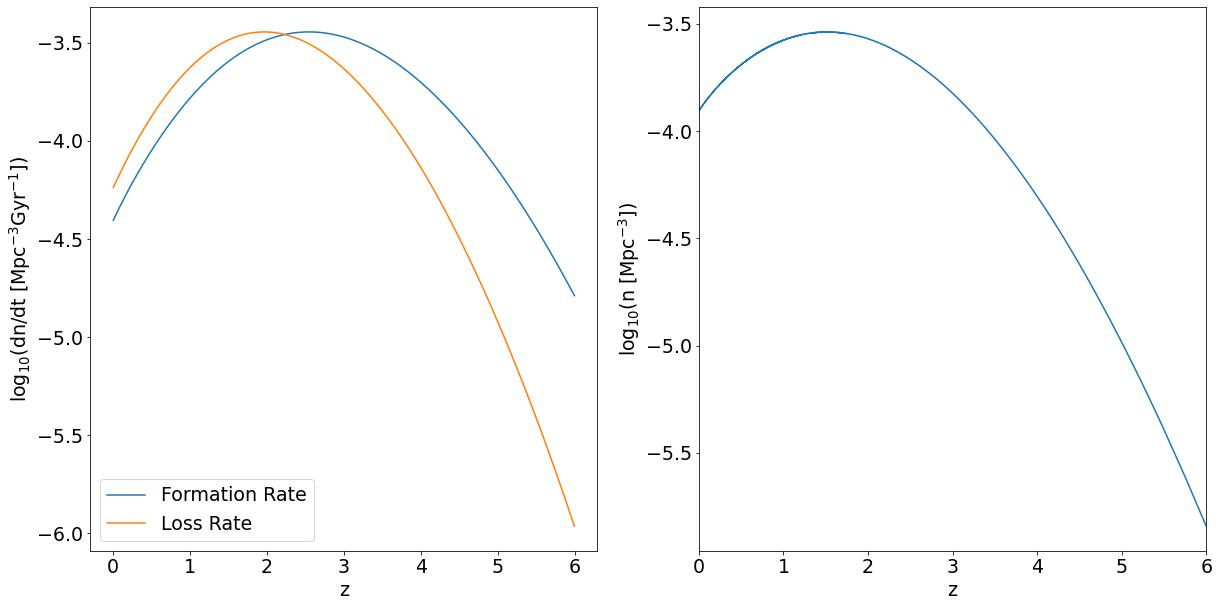
\includegraphics[width=\linewidth]{Plot_7_2.jpeg}
\caption{Left: Formation rate and loss rate of quasars as a function of redshift. The threshold halo mass for quasar formation is assumed here to have a constant value of $10^{12}M_\odot$. Right: Comoving number density of quasars as a function of redshift, calculated using Equation (8).}
\label{fig:7}
\end{figure}

\begin{figure}[H]
\centering
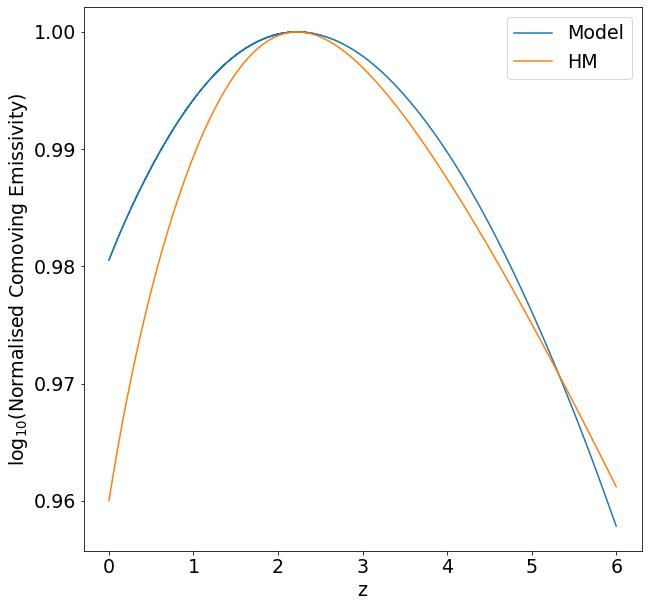
\includegraphics[width=12cm]{Plot_7_3.jpeg}
\caption{Comoving quasar emissivity as a function of redshift. The blue line shows the emissivity produced from our model using equation (10), and the orange line shows the emissivity at 912\AA \: calculated by \cite{Haardt_Madau} (Equation (11)). The emissivities peak at the same redshift and the model appears to be a good fit for the emissivity predicted by \citeauthor{Haardt_Madau} for $2\lesssim z\lesssim6$.}
\label{fig:8}
\end{figure}

\begin{figure}[H]
\centering
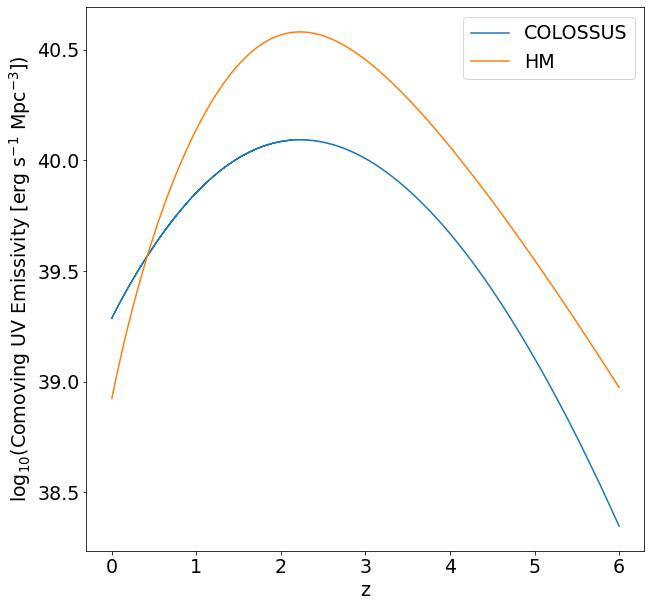
\includegraphics[width=12cm]{Plot_8.jpeg}
\caption{Comoving quasar UV emissivity as a function of redshift. The blue line shows emissivity calculated using Equation (15) and the orange line shows emissivity calculated from $\epsilon_{912}$ using Equation (13). The emissivity produced by our model is greater than $\varepsilon_{UV,HM}$ in this case.}
\label{fig:9}
\end{figure}

\twocolumngrid


\noindent alternative model for the case where quasar lifetimes are short and two alternative models which include a redshift-dependent $M_{H,crit}$.

\section{Investigating Alternative Models}

\subsection{Short Lifetime Case}

In the case where quasar lifetimes are small on the scale over which the formation rate varies, the comoving number density of quasars can be approximated as

\begin{equation}
    n\approx\frac{dn}{dt}\tau
\end{equation}

\noindent By substituting Equation (16) into Equation (15), obtain

\begin{equation}
    \varepsilon_{UV,Short}\approx\frac{dn}{dt}E_{UV}
\end{equation}

\noindent so the emissivity can be calculated without first obtaining the number density in this case, and is directly proportional to the quasar formation rate.\par

Comparing the plots in Fig.10 of quasar number density and UV emissivity produced using the short lifetime model with the initial model used in section 4 shows that this model's predictions are closer to the initial model than either of the models described in section 5.2. This model also appears to produce a similarly good fit for $\varepsilon_{UV,HM}$ to the initial model.

\subsection{Models with Variable Critical Mass}
\subsubsection{Keeping Virial Velocity Constant}

This model investigates the possibility that halos form quasars above a constant critical virial velocity, rather than a constant critical halo mass. The virial velocity of a halo is related to its mass by (\cite{Ikea})

\begin{equation}
    v_H^2=\alpha(GM_H)^{\frac{2}{3}}(10H)^{\frac{2}{3}}
\end{equation}

\noindent where $\alpha=\frac{3}{5}$. Rearranging this and setting $v_H=v_{H,crit}=constant$ gives

\begin{equation}
    M_{H,crit}(z)=\frac{v_{H,crit}^3}{10G\alpha^{\frac{3}{2}}}\frac{1}{H(z)}
\end{equation}

\noindent so $M{H,crit}$ decreases with redshift.\par

By comparing the plots from this model with the initial model in Fig.10, we see that this model produces significantly lower number densities of quasars and significantly lower UV emissivities than the initial model, with both being lower by approximately 1 order of magnitude. This is most likely because the constant virial velocity required to produce a good fit with $\varepsilon_{UV,HM}$ is $~300kms^{-1}$, which corresponds to a critical halo mass of $10^{13.3}M_\odot$ at $z=0$. This mass is significantly greater than the constant value used previously, and results in fewer halos crossing the mass threshold and forming quasars, which leads to the reduced magnitude of the emissivity.

\subsubsection{Star Formation-Driven Outflows}

In \cite{Quasar}, the buoyancy of outflows of gas from the galaxy driven by star formation is found to be dependent on the mass of the host halo. By comparing the 'adiabat' of the outflow to that of the host galaxy's diffuse corona, the critical halo mass, above which outflows would no longer be buoyant, is

\begin{equation}
    M_{H,crit}=M_0\Delta_z^{-\frac{3}{8}}
\end{equation}

\noindent where $M_0\sim10^{12}M_\odot$, and

\begin{equation}
    \Delta_z\equiv(\Omega_m(1+z)^3+\Omega_\Lambda)^{\frac{1}{3}}
\end{equation}

\noindent Above this critical halo mass, the outflows are trapped by the corona. Gas then builds up in the central regions of the galaxy, allowing

\onecolumngrid


\begin{figure}[H]
\centering
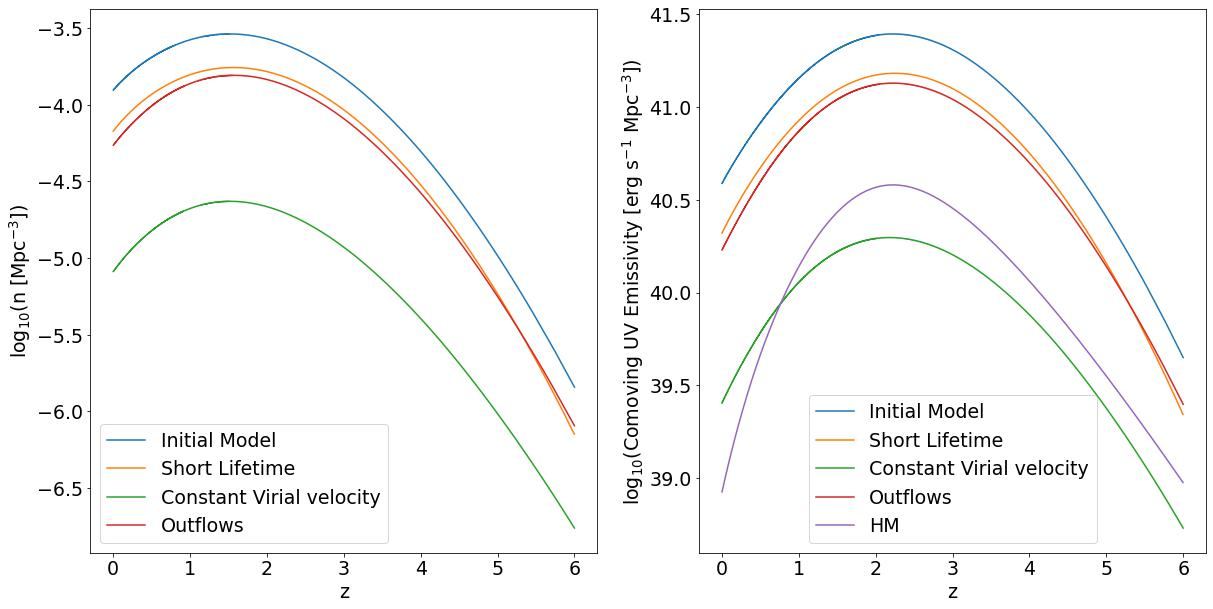
\includegraphics[width=\linewidth]{Plot_10.jpeg}
\caption{Left: Comoving number density of quasars plotted as a function of redshift. Produced using the initial model from section 4 (blue), the model with short quasar lifetimes (orange), the model where halos form quasars at a constant virial velocity (green), and the model where halos form quasars once star formation-driven outflows are no longer buoyant (red). All have been calculated using Equation (8), except for in the short lifetime model, which uses Equation (16). Right: Comoving quasar UV emissivity plotted as a function of redshift. Lines are coloured as on the left, where all have been calculated from the number densities on the left using Equation (15), except for in the short lifetime model, which uses Equation (17).The purple line shows the emissivity calculated from $\epsilon_{912}$ using Equation (13).}
\label{fig:10}
\end{figure}
\clearpage
\twocolumngrid


\noindent the SMBH to begin growing rapidly. As in the previous case, this leads to a critical halo mass which decreases with redshift.\par

Comparison of the plots in Fig.10 shows that, for $M_0=10^{12.4}M_\odot$, this model produces a similarly good fit for the evolution of $\varepsilon_{UV,HM}$ between redshifts 2 and 6 to the initial model, and produces quasar number densities and UV emissivities which are much closer to the constant $M_{H,crit}$ case than the model where virial velocity is kept constant. Additionally, this model produces very similar quasar number densities and emissivities to the short quasar lifetime model described in section 5.1.

 %The results shown so far have been produced using assumed values for $M{H,crit}$, $M_{BH,final}$, $\eta_{UV}$, and $k$ (the proportionality constant in Equation (7)) which are simple estimates. In the next section, we will investigate the effect of varying the values of $M{H,crit}$ and $k$ on the resulting emissivity, and determine values for $\zeta=\eta_{UV}M_{BH,final}$ which produce a good fit for the emissivity calculated from \citeauthor{Haardt_Madau}.

 %\section{Investigating the Effects of Changing Parameters}
 %\subsection{Varying $k$ and $M_{H,crit}$}

 %Hi.

%\section{Conclusions}

%The formation rate of quasars as a function of redshift has been calculated from the mass function of galaxies in the EAGLE Ref-L0100N1504 simulation which have crossed the mass threshold necessary to make the transition from the blue cloud to the red sequence and the logarithmic growth rate of galactic halos described by Correa et al. (2015). The quasar formation rate appears to peak at $z\approx1$.\par

%If the duration of the quasar phase after formation can be determined, the number of quasars present in the universe at a given redshift can be estimated. This has applications in developing a model for quasar evolution.

\bibliographystyle{mn2e.bst}
\bibliography{citation.bib}

\end{document}